\documentclass[twocolumn,10pt]{article}
\usepackage[a4paper, top=1.0in, bottom=1.0in, left=0.85in, right=0.85in]{geometry}

\usepackage{graphicx}
\usepackage{algorithm}  
\usepackage{algorithmicx}  
\usepackage{algpseudocode}  
\usepackage{amsmath}
\usepackage{url}

\renewcommand{\algorithmicrequire}{\textbf{Input:}}  
\renewcommand{\algorithmicensure}{\textbf{Output:}}  
\graphicspath{{figure/}}

\begin{document}

\date{}

\title{\bf Grouper: A Group Finance Manager on Mobile Devices Using Untrusted Servers}

\author{
	Meng Li, 201620728  
	\\ Supervisor: Yasushi Shinjo
}

\maketitle

\section{Introduction}
Conventional mobile applications are based on a client-server mode, which requires central servers for storing shared data. The users of such mobile applications must fully trust central servers and their application providers. Once a server is compromised by hackers, user information may be revealed because data is often stored on the server in cleartext. Finally, users may lose their data when service providers shut down their services. A group finance manager is an application that records the income and expenditure of a small group.

We are implementing a group finance manager application, Grouper, which is not relied on trusted central servers. This means user data cannot be cracked easily and its data can be recovered after services shutting down. A popular proposal is using P2P(Peer to Peer) to transfer user data between devices. However, there is a obvious problem in such a P2P proposal. Data transfer can only be finished during two devices are online at the same time. Another problem is that the number of P2P connections becomes large  fast as the number of users' increment. 

To address this problem, we use multiple untrusted servers for data transfer. Data will divided to several pieces and uploaded to diverse servers. Each server can only keep a piece of data temporarily. A piece will be deleted after a period time. Those two method can ensure that user data cannot be cracked easily. In addition, all devices of group members keep a complete data set, data can be recovered even untrusted servers shut down.

\section{Design}

We design a group finance manager application, Grouper, on mobile devices, which is not relied on trusted central servers. 

\subsection{Group Finance Manager}
 In Grouper, group members can create a record including money, classification, account, shop, remark and time. With data synchronization, they can also share their records with other group members, so that group income and expenditure information can be analyzed and shown to all members. Grouper uses multiple untrusted servers to synchronize and avoids relying on trusted central servers. To create a group in Grouper, the owner of this group needs to register and set an access key in untrusted servers. The owner passes the access key to group members by a face-to-face way.

\subsection{Shamir's Secret Sharing}
Secret sharing creates a numbers of shares and plays an indispensable role in protecting user data from getting lost or destroyed. In a secret sharing scheme, a dealer securely shares a secret with a group of participants, by generating $n$ shares using a cryptographic function\cite{smith2013layered}. At least $k$ or more participants can reconstruct the secret, but $k-1$ or fewer participants can obtain nothing about the secret\cite{pang2005new}. We describe this scheme as a function $f(k, n)$, where n is the number of all shares, and k is the threshold to combine shares.  Shamir's Secret Sharing is a popular technique to implement threshold schemes.

\subsection{Data Synchronization Using Multiple Untrusted Servers}

We design Grouper based on data synchronization by multiple untrusted servers rather than a single server. There are three principles in our proposal. 

Firstly, a server transfers data, does not keep it permanently. Most current popular client-server applications store user data on several central servers, user data will not be deleted unless user deletes his account. Grouper uses untrusted servers as a bridge for transferring data. Consider that a group include three members: Alice, Bob and Carol. Alice creates a new record in her device, this record is uploaded to untrusted servers, and the record on servers will be eliminated after Bob and Carol download it from servers.

Secondly, a server keeps data temporarily. We define a period of time in which data can be kept in a server. In this paper, we set this period to 1 hour for our example situations. The record Alice uploaded to untrusted servers can only exist for 1 hour. After 1 hour since uploaded, this record will be deleted. Alice requires to resend this record to serves until all of other members has downloaded successfully. However, the longer keeping period means the higher risk of data reveal. The most suitable period is influenced by the number of group members, security requirement and others. 

Thirdly, servers do not know the content of data. Keeping data temporarily cannot ensure data security, because servers know the cleartext of data in this temporary period. For this problem, developers often encrypt data before uploading to servers, and this needs a key to decrypt data in other devices. In order to distribute the private key, users should share it by themselves. In this paper, we use secret sharing, which can create a number of shares and distributing them to a set of participants\cite{smith2013layered}, to share data between user devices.

\begin{figure}[t]
\centering
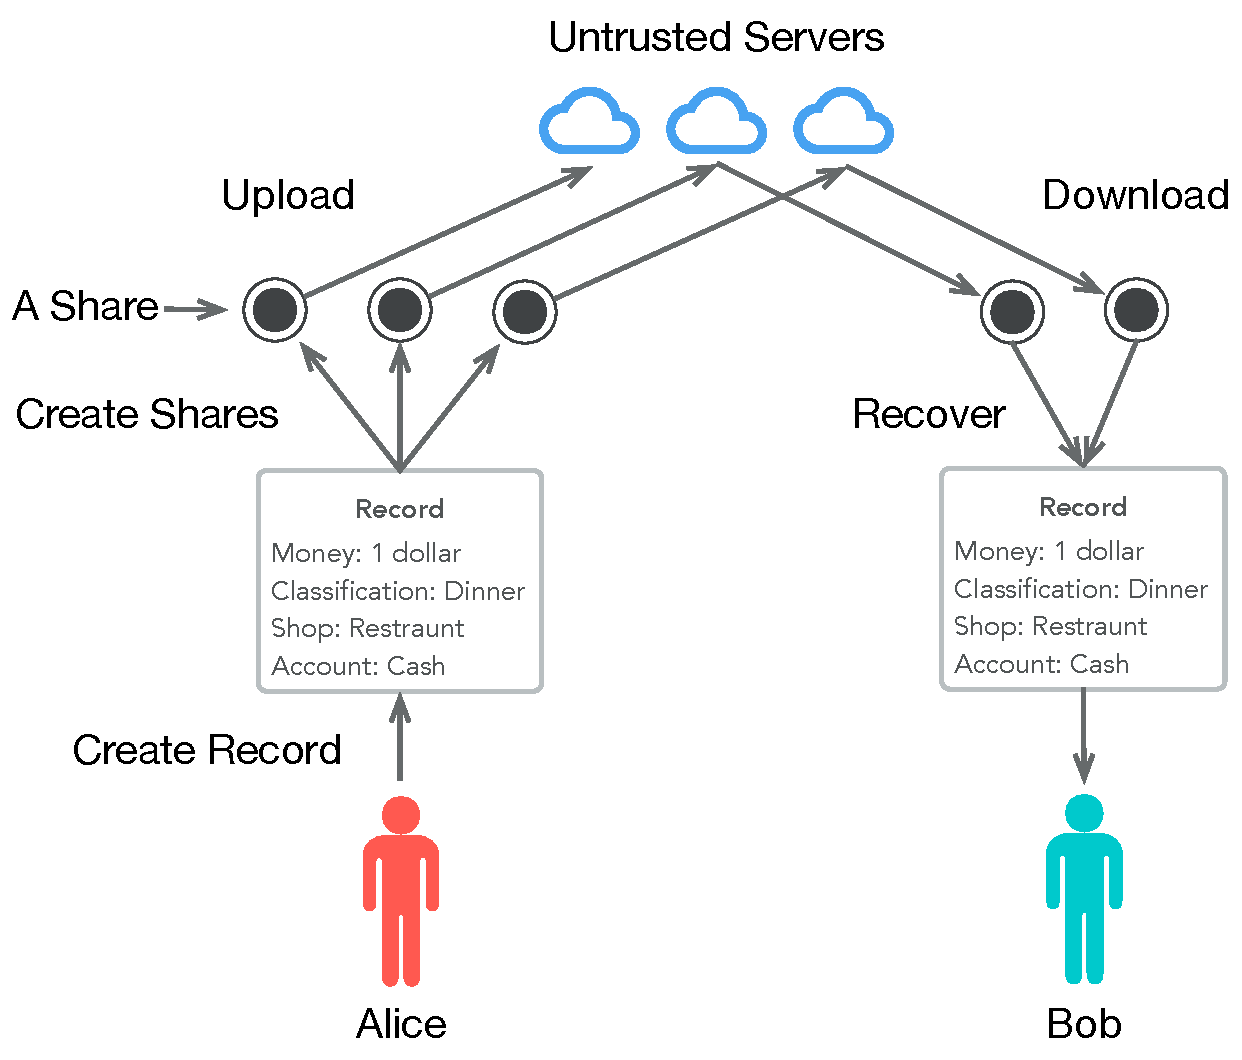
\includegraphics[scale=0.35]{sync_flow}
\caption{Flow of Synchronization}
\end{figure}

Figure 1 describes our synchronization flow based on the three core principles. At first, Alice adds a record and Grouper creates a number of shares by secret sharing. Next, Grouper uploads those shares to multiple untrusted servers. When Bob is online, Grouper in Bob's device downloads shares from servers and recover the new record created by Alice. In this situation, Grouper can recover the record after getting more than two shares. In this process, each server is separated from other servers, and cannot access to other servers. This means that user data can not be recovered unless some entity has permission to access these untrusted servers. In our proposal, only group members have permission to access these untrusted servers.

\subsection{Reliable Synchronization}
Grouper should provide a reliable synchronization service. For example, once Alice, who is a user in a group, creates a new record in her device, all of other members in a group should synchronize this record, even if this record may be deleted by untrusted servers after a period of time. We call this problem \emph{Reliable Synchronization}.

Figure 2 describes the situation data cannot be synchronized completely. Alice sends a new record to untrusted servers at 10:00 AM and Bob downloads it successfully at 10:30 AM. Carol downloads failed after 11:00 AM because the shares of this record has been deleted by servers. To solve this problem, Alice should upload her new record again until Carol downloads it successfully. However, it is hard for Alice to get the information that all of other members in her group have download. We must find an efficient way for notifying Alice that all members have synchronized successfully.

\begin{figure}[t]
	\centering
	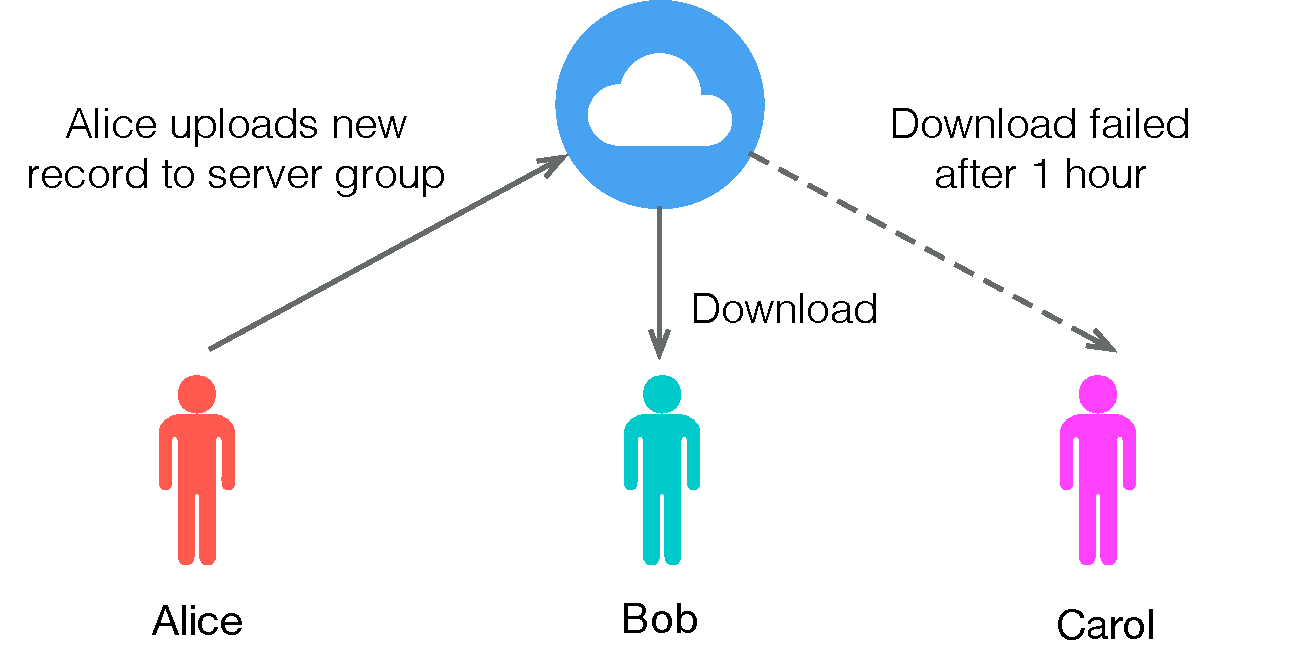
\includegraphics[scale=0.35]{unreliabe_sync}
	\caption{Unreliable Synchronization}
\end{figure}

We are designing a single method to solve this problem. This method uses a counter in clients as the solution to the \emph{Reliable Synchronization} problem. Intuitively, this counter calculates the number of times other clients synchronized and works on the sender to decide resending record or not. The condition that sender device needs not to resend a record can be described as Equation 1:
\begin{equation}
\sum_{i=1}^{n}s_{i}=(m-1)\cdot k
\end{equation}

In Equation 1, we suppose that there are $n$ untrusted servers, Server 1, Server 2,..., Server $n$. This is also the first parameter, the number of all shares, in the scheme $f(k, n)$ of Shamir's secret sharing. Each server keeps a share, so $n$ servers saves $n$ shares. Each server should know how many times the share has been downloaded by clients. Thus, we use $s_i$ to represent the number of download times in server $i$. The sum of $s_i$ is calculated in the sender client. In the left of Equation 1, $m$ represents the number of group members, and $k$ is the threshold in scheme $f(k, n)$. Obviously, a client can reconstruct data after getting $k$ shares. If $m-1$ clients have reconstructed data, $(m-1)\cdot k$ shares is downloaded. That means clients except sender has synchronized successfully, so the sender need not to upload again.

To implement such a counter, restriction about security and connection should be considered. Remember that servers do not communicate with each other. Actually, one server of the group does not know the others in the group. On the other hand, clients cannot communicate with each other. Clients do not know IP address or domain name of other device, so that they cannot send messages with P2P connections. To address this problem, we design the sender table in clients and the transfer table in servers described as shown in Figure 3. 

\begin{table}[tbp]
	\centering  
	\begin{tabular}{lll}  
		\hline
		Column &Data Type & Introduction\\ 
		\hline  
		sid &String & Physical unique identifier\\
		content & String & JSON String of object\\ 
		object & String & Name of object\\
		count & Integer16 & Count of sync time\\
		resend & Boolean &Necessity of resending data \\
		sendtime & Date & Data send time\\
		\hline
	\end{tabular}
	\caption{Columns of Sender Table}
\end{table}

Columns of a sender table are listed in Table 1. Here, sid, content, and count of sync times are main columns. The column  sid is an unique identifier created by a database in a client, it is same as those in servers. The column content saves the JSON string generated from a record object. The column count has the sync times of this object. In a server, a transfer table also has these three main columns with different meaning. The column sid is equals to that in a client in order to identify the row corresponding to that in the client. The column content has one of the shares generated by secret sharing scheme. The column count has the number of content sync times in server.

\begin{figure}[t]
	\centering
	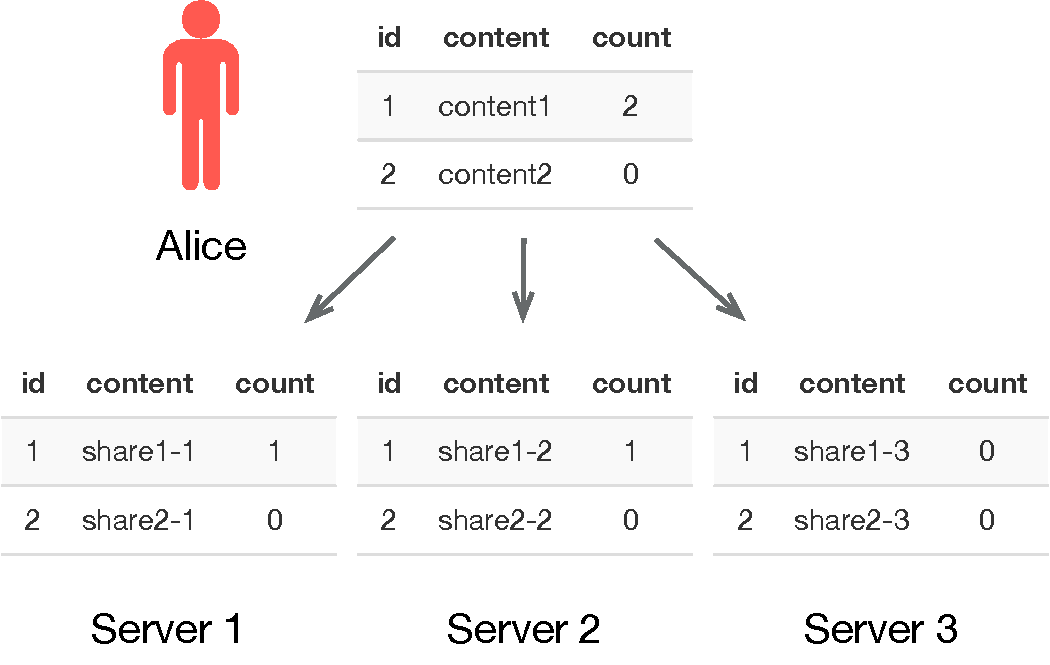
\includegraphics[scale=0.4]{sync_table}
	\caption{Sender Table and Transfer Table}
\end{figure}

In Figure 3, suppose that the secret sharing scheme is $f(2, 3)$, and only Bob has synchronized Alice's new record within a prescribed time period. The column corresponding to Alice's new record, whose id is 1, is equals to those columns whose ids are 1 in Server 1 and Server 2. This means that Bob downloaded two shares from Server 1 and Server 2. The client of Alice will know that by responses from Server 1 and Server 2 when it upload data again. It will upload for one more time, because it's count is 2. This is less than 4, the threshold Alice needs not to upload again.

However, if we consider a further problem that Carol, who is offline, can attack this group by being lazy. Alice, the record creator, has to upload shares to untrusted servers indefinitely. We are addressing this problem now by holding a list group members in untrusted servers.

\section{Implementation}
Grouper consists of an iOS application for clients and a Web service in servers.

\subsection{Client}
In Section 2, we have introduced how to sharing a string with other deices via multiple untrusted servers. In this section, we first describe persistent store and data synchronization. Grouper stores all data on mobile devices with an object-oriented way. Grouper uses Core Data\cite{coredata}, a native iOS framework to manage the model layer objects. Core Data provides generalized and automated solutions to common tasks associated with object life cycle and object graph management, including persistence. Sync\cite{sync} by Elvis Nu\~{n}ez is a modern JSON synchronization framework to Core Data, helps data synchronization in Grouper by parsing a JSON response and getting it into Core Data. With Sync based on Core Date, we can concentrate on sharing with untrusted servers rather than data storage and synchronization.

In this paper, we use c-SSS\cite{c-sss}, an implementation in original C code of Shamir's Secret Sharing by Fletcher T. Penney. This implementation supports UTF-8 character set without limitation of length. It provides two main functions including \emph{generate}, which generates $n$ shares by the string text with the threshold $k$, and \emph{extract}, which recreates the text string after accessing to more than $k$ shares. c-SSS generates shares from a JSON string. There shares are stored into the sender table. Grouper generates shares and send them by a REST API to servers until this record is synchronized successfully by all of other group members.

\begin{figure}[t]
\centering
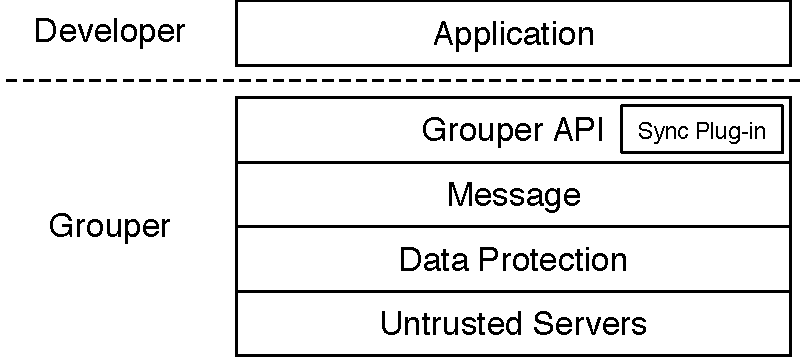
\includegraphics[scale=0.35]{architecture}
\caption{Architecture of Client}
\end{figure}

\subsection{Web Service}
Many applications with synchronization is based on commercial cloud services like Amazon S3 or Google Cloud. Grouper needs its own Web service rather than using commercial general cloud services for following reasons:

\begin{itemize}
\setlength{\itemsep}{1pt}
\setlength{\parskip}{0pt}
\setlength{\parsep}{0pt}
	\item Web service should have a counter to calculate the number of sync times.
    \item Web service should ensure that a share can be delete after a prescriptive time.
    \item Only group members who has an access key can download shares from servers. In other word, a Web service plays a role of access control.
\end{itemize}

\section{Related Work}

DepSky\cite{bessani2013depsky} is a system that stores encrypted data on servers and runs application logic on the client-side\cite{wang2016sieve}. DepSky provides a storage service that improves the availability and confidentiality provided by commercial storage cloud services. \emph{Cloud-of-Clouds} is the core concept in DepSky. It represents that DepSky is a virtual storage cloud, which is accessed by its users by invoking operations in several individual severs. DepSky keeps encrypted data in commercial storage cloud services and do application logic in individual servers. In Grouper,  untrusted servers undertake responsibility of temporarily data storage and message delivery with server-side computation.

Mylar\cite{popa2014building} stores encrypted and sensitive data on the server, and decrypts this data only in users’ browsers. Developers of Mylar use its API to encrypt a regular(non-encrypted) Web application, and users decrypt data by a browser extension. Like Grouper, applications in Mylar can control how user data is shared\cite{wang2016sieve}. Unlike Grouper, Mylar builds its system on a browser with browser extension while Grouper uses mobile device as a client.

There are many applications or frameworks that use untrusted network and servers. Compared to them, Grouper uses secret sharing and temporary data storage with untrusted servers to protect user data from malicious attacking. It is convenient and faster compared to those applications or frameworks using data encryption for the reason that Grouper uses Secret Sharing to hide the cleartext.

\section{Conclusion}

This paper introduces Grouper, a group finance manager that synchronizes with multiple untrusted servers. Grouper uses Secret Sharing and temporary data storage on mobile devices. Grouper consists of an iOS application and a Web service.  Each server of Grouper does not know the others and keeps one of the shares generated by secret sharing temporarily, to ensure that user data cannot be cracked easily. We are developing an application running in a iOS device and a Web service running on Tomcat server. We connect these clients and multiple untrusted servers by REST API.

\bibliographystyle{unsrt}
\bibliography{ref}

\end{document}
